\chapter{Machine Learning in Particle Physics}
\label{chap:machine-learning}
Since this work focuses on improving the event reconstruction of dileptonic \ttbar decays using machine learning techniques, this chapter aims to provide an overview over the fundamental concepts and methodologies employed in machine learning.

From a computational perspective, machine learning can be viewed as the optimisation of a function $f:\mathbb{R}^n \rightarrow \mathbb{R}^m$ that maps input data points $\mathbf{x} \in \mathbb{R}^n$ to output predictions $\mathbf{y} \in \mathbb{R}^m$. The function $f$ is parameterised by a set of learnable parameters $\theta$, which are adjusted during the training process to minimise a predefined \textit{loss function} $L(\mathbf{y}, f(\mathbf{x}; \theta))$. The loss function quantifies the discrepancy between the predicted outputs and the true target values, guiding the optimisation process.


\section{Supervised Learning}
Machine learning can be broadly categorised into supervised and unsupervised learning. In supervised learning, the model is trained on a labelled dataset, where each input data point is associated with a corresponding target output. The goal of the model is to learn a mapping from inputs to outputs, enabling it to make accurate predictions on unseen data.


\subsection{Monte Carlo Training Data}
\begin{figure}
    \centering
    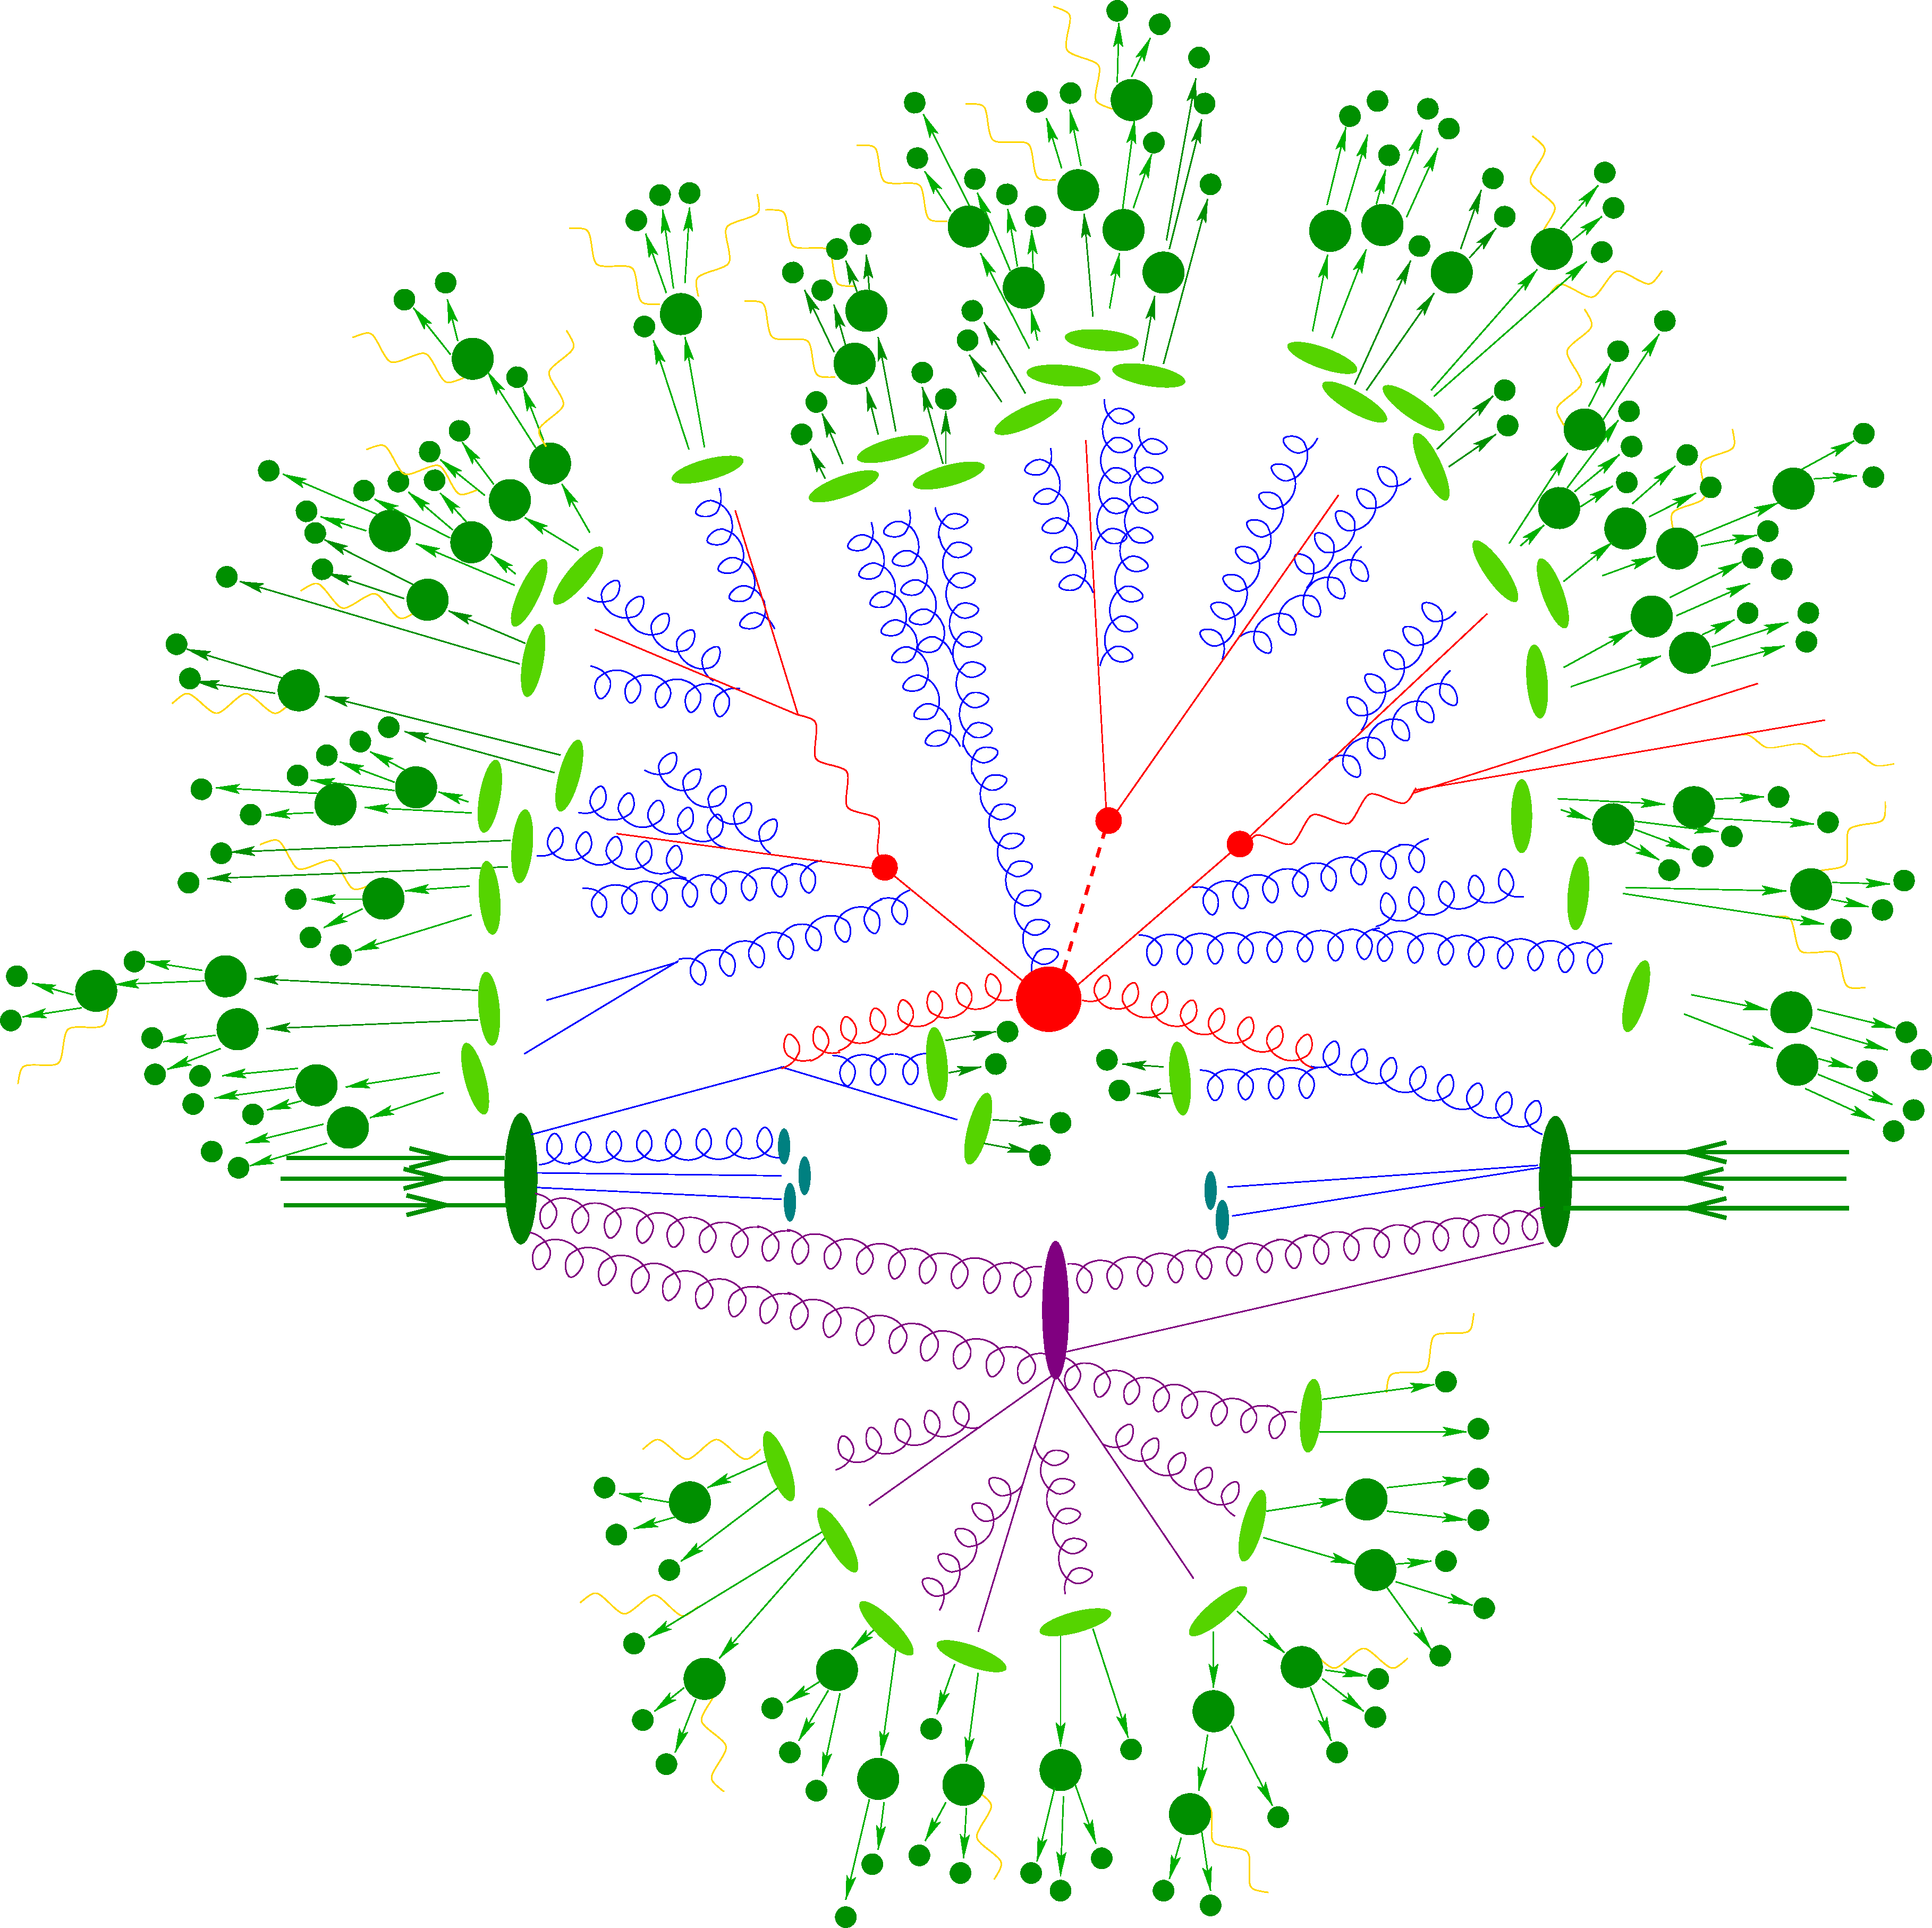
\includegraphics[width=0.6\textwidth]{figures/event_svg-tex.pdf}
    \caption{Schematic representation of the Monte Carlo event generation process in particle physics. Colouring of vertices and particles indicates the event generation stage: hard scattering process (big red blob), QCD radiation (blue), hadronisation (light green), showering (dark green), and a secondary vertex (purple). The Figure is taken from Reference~\cite{sherpa_1}.}
\end{figure}
\label{sec:mc_training_data}
Events are usually simulated using a cascade of different programs, each simulating a different state of the event. First the hard scattering process is simulated using matrix element generators. These programs calculate the probabilities of different particle interactions based on the underlying physics theories, such as the Standard Model. Using these probabilities, they generate events that represent the initial state of the particles after the collision. The possible kinematic phase space is sampled according to these probabilities, resulting in a set of particles with specific momenta and energies. This type of event variables is often referred to as \textit{parton-level}.

Next, the parton showering and hadronization processes are simulated. Parton showering models the emission of additional particles from the initial partons, while hadronization simulates the formation of hadrons from quarks and gluons. These processes are crucial for accurately modelling the final state particles observed in detectors.

Finally, detector simulation programs are used to simulate the interaction of particles with the detector material, producing realistic detector responses. This includes simulating the energy deposits in calorimeters, hits in tracking detectors, and other relevant signals.

While the actual detector response is simulated using complex detector simulation software, for many machine learning applications, a simplified representation of the detector response is sufficient. This can involve smearing the particle momenta and energies according to the detector resolution, applying efficiency corrections, and simulating the effects of pile-up.

This is because, for the reconstruction of the physics objects, such as jets, leptons, and missing transverse energy, highly sophisticated algorithms are used that already take into account the detector effects (Note that these algorithms may also be machine learning based). Therefore, the input features for machine learning models can often be derived directly from these reconstructed objects, rather than relying on the raw detector signals. The reconstructed object event variables are called \textit{reco-level}.

\subsection{Training}
During the training phase, the model is presented with a set of input features derived from the reco-level event variables, along with their corresponding target outputs, which are typically derived from the parton-level event variables. The model learns to map the input features to the target outputs by minimizing a loss function that quantifies the difference between the predicted and true values. Common loss functions include mean squared error for regression tasks and cross-entropy loss \cite{cross-entropy} for classification tasks.
The training process involves iteratively (each step is called \textit{epoch}) updating the model's parameters using an optimisation algorithm to minimise the loss function.

\subsection{Validation and Testing}
To evaluate the performance of the trained model, it is essential to validate and test it on independent datasets that were not used during training. This helps to assess the model's generalization capabilities and ensures that it can make accurate predictions on unseen data. A common practice is to split the available data into training, validation, and test sets. The validation set is used to tune hyperparameters and monitor the model's performance during training, while the test set is reserved for the final evaluation of the model's performance.

Since in particle physics, simulated data is often used for training and background modelling, one typically employs a k-folding strategy \cite{k-folding}, where the data is divided into k subsets. The model is trained k times, each time using a different subset as the validation set and the remaining subsets for training. This approach helps to use the available data more efficiently.

\section{Regression and Conditional Density Learning}
To highlight some important distinctions between different machine learning tasks, it is useful to briefly discuss regression and conditional density learning.
\subsection{Supervised Learning as Risk Minimisation}
In supervised learning, the goal is to learn a parametrised function $f_\theta$ that maps input data $\mathbf{x}$ to output predictions $\mathbf{y}$. This can be formalised as a risk minimisation problem, where the objective is to minimise the expected loss over the joint distribution of inputs and outputs. The expected risk can be expressed as:
\begin{equation}
    R(f) = \mathbb{E}_{\mathbf{x}, \mathbf{y}}[L(\mathbf{y}, f_\theta(\mathbf{x}))]
\end{equation}
where $L$ is the loss function that quantifies the discrepancy between the true output $\mathbf{y}$ and the predicted output $f_\theta(\mathbf{x})$. The goal of training is to find the parameters $\theta$ that minimise this expected risk, which is typically approximated using empirical risk minimisation on the training dataset.
\subsection{Regression}
In regression tasks, the output $\mathbf{y}$ is a continuous variable, and the model is trained to predict a specific value for each input $\mathbf{x}$. The loss function commonly used for regression is the mean squared error (MSE), which measures the average squared difference between the predicted values and the true values:
\begin{equation}
    L_{\text{MSE}}(\mathbf{y}, f(\mathbf{x})) = \frac{1}{N} \sum_{i=1}^{N} (y_i - f_\theta(\mathbf{x}_i))^2
\end{equation}
where $N$ is the number of samples in the dataset. The model learns to minimise this loss function. If the labels are not deterministic, meaning that there is inherent uncertainty in the target values, one can describe the labels using a conditional probability distribution $p(\mathbf{y}|\mathbf{x})$. In this case, minimising the MSE corresponds to learning the conditional mean of the distribution (see \Cref{chap:supplementary_computations_and_proofs} for a proof):
\begin{equation}
    f_\theta(\mathbf{x}) = \mathbb{E}[\mathbf{y}|\mathbf{x}] = \int \mathbf{y} p(\mathbf{y}|\mathbf{x}) d\mathbf{y}\,.
\end{equation}
Depending on the loss-function used, the model can learn different statistics of the conditional distribution. For example, using the mean absolute error (MAE) loss function would lead to learning the conditional median instead of the mean.

\subsection{Conditional Density Learning}
In contrast to regression, conditional density learning aims to learn the entire conditional probability distribution $p(\mathbf{y}|\mathbf{x})$ rather than just a point estimate. This is particularly useful when the target variable has inherent uncertainty or when multiple outcomes are possible for a given input. To quantify the difference between the true conditional distribution and the model's predicted distribution, the Kullback-Leibler (KL) divergence is often used as a loss function \cite{kl_divergence}
\begin{equation}
    L_{\text{KL}}(p, q) = \int p(\mathbf{y}|\mathbf{x}) \log \left( \frac{p(\mathbf{y}|\mathbf{x})}{q_\theta(\mathbf{y}|\mathbf{x})} \right) d\mathbf{y}
\end{equation}
where $p(\mathbf{y}|\mathbf{x})$ is the true conditional distribution and $q_\theta(\mathbf{y}|\mathbf{x})$ is the model's predicted distribution. Minimizing this loss function encourages the model to produce a predicted distribution that closely matches the true distribution, allowing for a more comprehensive understanding of the uncertainty and variability in the target variable. In practice, computing KL divergence can be challenging, since the true distribution might be unknown or difficult to estimate. In such cases, one relies on the data to provide an empirical estimate of the true distribution, and the loss function is approximated using samples from the dataset. It can be shown that minimizing the KL divergence is equivalent to maximizing the likelihood of the observed data under the model's predicted distribution, which is a common approach in training probabilistic models. For the case of a discrete target variable, this corresponds to minimising the cross-entropy loss, which is widely used in classification tasks \cite{cross-entropy}.

\section{Neural Networks}
\begin{figure}[ht]
    \centering
    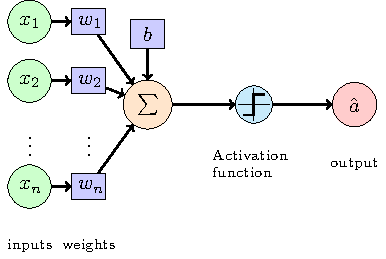
\includegraphics[width=0.6\textwidth]{figures/machine-learning/perceptron.pdf}
    \caption{Schematic of a single artificial neuron (perceptron). The neuron receives multiple input signals, each associated with a weight, and computes a weighted sum of these inputs, optionally a so-called bias is added. An activation function is then applied to this sum to produce the neuron's output.}
    \label{fig:perceptron}
\end{figure}
As elaborated before, machine learning models can be viewed as parameterised functions that map input data to output predictions. Neural networks are a class of machine learning models that are inspired by the structure and function of biological neural networks in the human brain. They consist of interconnected artificial neurons that process and transform the input data to produce the desired output.
The simplest unit of a neural network is the artificial neuron, also known as a perceptron \cite{perceptron}. A perceptron takes multiple input signals, each associated with a weight, and computes a weighted sum of these inputs. An activation function is then applied to this sum to produce the neuron's output. This structure is illustrated in \Cref{fig:perceptron}. The general structure of a perceptron is inspired by biological neurons. The activation function introduces non-linearity into the model, allowing it to learn complex patterns in the data. Common activation functions include the sigmoid function, hyperbolic tangent (tanh), and rectified linear unit (ReLU) \cite{relu}. For this work, the ReLU activation function is used, which is defined as $f(x) = \max(0, x)$, meaning that it outputs the input directly if it is positive, and zero otherwise. This activation function has been shown to be effective in training deep neural networks by mitigating the vanishing gradient problem \cite{relu}.


\subsection{Dense Neural Network}
\begin{figure}[ht]
    \centering
    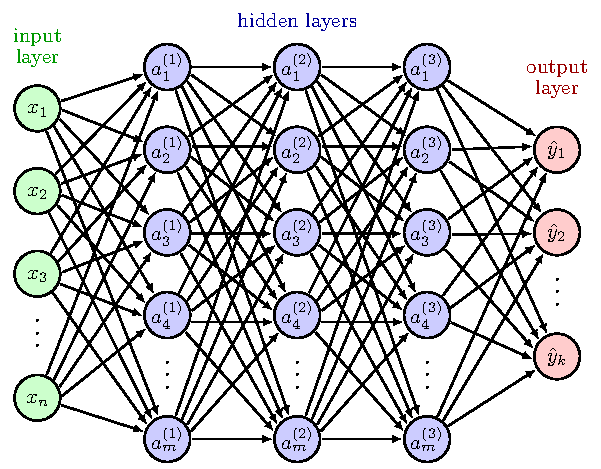
\includegraphics[width=0.5\textwidth]{figures/machine-learning/dnn.pdf}
    \caption{Schematic of a dense neural network with multiple layers. Each layer consists of multiple neurons, and each neuron in one layer is connected to every neuron in the subsequent layer.}
    \label{fig:dnn}
\end{figure}
A dense neural network (DNN), also known as a fully connected neural network \cite{backpropagation}, is a type of artificial neural network where each neuron in one layer is connected to every neuron in the subsequent layer. This architecture allows for the learning of complex relationships between input features and output targets. A schematic of a dense neural network is shown in \Cref{fig:dnn}.

A DNN consists of an input layer, one or more hidden layers, and an output layer. The input layer receives the input features, while the hidden layers perform a series of transformations on the data using the weights and biases associated with each neuron. The output layer produces the final predictions. Each layer applies an activation function to the weighted sum of inputs from the previous layer, enabling the network to learn non-linear mappings. The depth (number of layers) and width (number of neurons per layer) of the network can be adjusted.

\subsection{Transformer Networks}
\label{sec:transformer}
\begin{figure}[ht]
    \centering
    \begin{subfigure}[b]{0.3\textwidth}
        \centering
        \includegraphics[scale = 0.71]{figures/machine-learning/dpa.pdf}
        \caption{\centering Scaled \\ Dot-Product Attention}
        \label{fig:dpa}
    \end{subfigure}
    \begin{subfigure}[b]{0.35\textwidth}
        \centering
        \includegraphics[scale = 0.71]{figures/machine-learning/mha.pdf}
        \caption{Multi-Head Attention}
        \label{fig:mha}
    \end{subfigure}
    \begin{subfigure}[b]{0.3\textwidth}
        \centering
        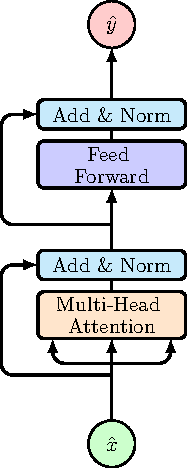
\includegraphics[scale = 0.71]{figures/machine-learning/transformer_layer.pdf}
        \caption{Transformer Layer}
        \label{fig:transformer_layer}
    \end{subfigure}
    \caption{Different components of the transformer architecture from smallest to largest unit: (a) Scaled Dot-Product Attention, (b) Multi-Head Attention, and (c) Transformer Layer.}
    \label{fig:attention}
\end{figure}
The transformer architecture deals with sequential data using an attention mechanism. This allows transformers to process information in parallel, making them efficient for training on large datasets. Additionally, transformer can capture long-range dependencies in the data very effectively, as they relate all elements of the input sequence to each other through attention mechanisms.

The core component of the transformer architecture is the attention mechanism, which allows the model to focus on different parts of the input sequence when making predictions. The most commonly used attention mechanism is the scaled dot-product attention \cite{attention_is_all_you_need}, illustrated in \Cref{fig:dpa}. In this mechanism, three vectors are computed for each input element: the query ($q$), key ($k$), and value ($v$) vectors. The attention scores are calculated by taking the dot product of the query and key vectors, scaling them by the square root of the dimension of the key vectors, and applying a softmax function to obtain attention weights. These weights are then used to compute a weighted sum of the value vectors, producing the output of the attention mechanism.
Multi-head attention, shown in \Cref{fig:mha}, extends the scaled dot-product attention by allowing the model to attend to different parts of the input sequence simultaneously. This is achieved by using multiple parallel attention heads, each with its own set of learned linear transformations for the query, key, and value vectors. The outputs of all attention heads are concatenated and linearly transformed to produce the final output.

The key, query and value vectors are typically obtained by applying learned linear transformations to the input embeddings. Depending on the type of relational information one wants to capture, one can choose to derive these vectors from different input sources. For example, in the \textit{self-attention mechanism}, all three vectors are derived from the same input sequence ($\hat q_t = \hat k_t=\hat v_t = \hat x_t$), allowing the model to relate different elements within the same sequence. In \textit{cross-attention}, the query vectors are derived from one sequence, while the key and value vectors are derived from another sequence ($\hat q_t = \hat x_{1,t}$, $\hat k_t=\hat v_t = \hat x_{2,t}$), enabling the model to relate information between two different sequences.
\paragraph{Symmetries}
In many applications, including particle physics, the input data exhibits certain symmetries that can be exploited to improve model performance.

The attention mechanism has inherent permutation equivariances, that can be exploited. Self-attention is permutation equivariant to the input sequence, meaning that permuting the input elements results in a corresponding permutation of the output elements. This property is particularly useful when dealing with sets or unordered data, where the order of the elements does not carry any inherent meaning. Cross-attention is permutation equivariant to permutations of the query inputs and separately to permutations of the key/value inputs. This allows the model to effectively relate information between two different sequences, regardless of their order.

\subsection{Training Neural Networks}
Training neural networks involves optimizing the model's parameters (weights and biases) to minimise the loss function. The number of parameters in a neural network can rise rapidly, especially in deep architectures, making the optimisation process computationally intensive. The most commonly used optimisation algorithm for training neural networks is stochastic gradient descent (SGD) \cite{sgd}, which iteratively updates the model's parameters based on the gradients of the loss function with respect to the parameters. Modern variants of SGD, such as Adam \cite{adam}, incorporate adaptive learning rates and momentum to improve convergence.
The backpropagation algorithm \cite{backpropagation} is used to efficiently compute the gradients of the loss function with respect to the model's parameters. It involves propagating the error signal backward through the network, allowing for the calculation of gradients at each layer. These gradients are then used by the optimisation algorithm to update the parameters. The algorithm relies on the chain rule and nested structure of the neural network to compute the gradients efficiently.
Regularization techniques, such as dropout \cite{dropout} and weight decay, are often employed during training to prevent overfitting and improve the model's generalization capabilities. Dropout randomly deactivates a fraction of the neurons during training, forcing the network to learn more robust features. Weight decay \cite{adamW} adds a penalty term to the loss function based on the magnitude of the weights, discouraging overly complex models and promoting generalization.